% EJB
\ifbook{
    \mysubsubsection{Propos de cette section}

    \paragraph{} Comme l'a explicité, dans les premiers chapitres, la description des nombreux
    "conteneurs d'exécutions" dans lesquelles les applications modernes sont déployées. Un grand
    nombre de mécanismes, associés aussi à des certaines contraintes de programmation donne un
    cadre puissant et robuste à l'application.

    \paragraph{} Malgré tout ceci, la réalisation d'application reste un sujet vaste, et il
    est fréquent que, dans le cadre d'un projet, on décide d'utilise un ou plusieurs autres
    \textit{frameworks} supplémentaires, fournissant généralement un cadre de développement estimé
    encore plus efficase ou approprié pour l'implémentation désirée.

    \paragraph{} Rien que dans le monde Java, on distingue une kyrielle vertigineuse de ces
    \textit{frameworks} parmi lesquelles on citera juste les suivants, à titre d'exemple:

    \begin{itemize}
      \item \mylink{http://www.springsource.org/}{Spring}: un \textit{framework} très souvent
      utilisé et conçu pour offrir un cadre robuste, simple et complet aux développement
      d'applications \textit{web} modernes. Il est souvent présenté comme une alternative plus
      simple à l'utilisation des standards associés à JEE.
      \item \mylink{http://struts.apache.org/}{Struts}: un très célèbre \textit{framework} adaptant
      le classique modèle
      \mylink{http://fr.wikipedia.org/wiki/Mod\%C3\%A8le-Vue-Contr\%C3\%B4leur}{MVC} à la
      réalisation d'application \textit{web}.
      \item \mylink{http://www.oracle.com/technetwork/java/javaee/javaserverfaces-139869.html}{JSF}
      et ses implémentations: standard issu du monde JEE, JSF propose un modèle de programmation
      dédié à la réalisation d'application \textit{web} métiers. Un des objectifs avoués du standard
      et de ses implémentations est de permettre un développement similaire à celui d'application
      dites "lourdes", en prenant en charge, autant que possible, les spécificités des technologies
      internet.
      \item ...
   \end{itemize}

   \paragraph{} Fort de ce simple constat, il apparait évident que dresser un tabelau exhaustif,
   même limiter à l'univers Java/JEE Open Source et standard, formerait une excellente treizième
   tâche pour Hercule, et dépasserait totaltement le cadre de cet exposé.

   \paragraph{} Néanmoins, ce genre de composant formant une partie intégrante du paysage associé
   aux \textit{middleware}, il est pertinent, dans le cadre de ce cours, de présenter l'un d'eux. Cette
   analyse donnera, espérons-le, au lecteur, une grille de lecteur suffisante pour entreprendre lui
   même ce travail de "décorticage" technologique lorsqu'il sera confronté à la toute dernière
   déclinaison "à la mode" de ces \textit{frameworks}.

   \paragraph{} Cette section présente donc, de manière volontairement très sommaire, les grandes
   lignes du modèle de programmation promût par le standard EJB, dans sa troisième version (de loin
   à ce jour la plus simple et réussie). L'objectif de ce standard, et de ses implémentations, est
   donc - comme nous allons le voir, la normalisation de la définition et de l'utilisation de
   \textbf{composant distribué}.

   \paragraph{} \textit{Le lecteur prendra soin de noter immédiatement l'importance de bien saisir
   quel est l'objectif que cherche à atteindre le framework et quel modèle de programmation
   il promeut. En effet, il est, de manière très regrettable, fréquent de
   voir des projets embarqués une kyrielle de composants, plus ou moins standard, plus ou moins
   ouvert, plus ou moins robustes, mais surtout plus ou moins utile à l'application. Cette
   empilement technologique confus, au delà de rendre le code de l'application très complexe, a
   aussi l'effet de bord d'augmenter grandement la difficulté de sa mise en oeuvre.}

   \mysubsubsection{Motivations et objectifs des EJB}

   \paragraph{} L'objectifs du standard EJB est de définir un ensemble d'API pour faciliter et
   normaliser la conception de composant \textbf{distribué}, et de permettre ainsi de construire
   des applications où les traitements sont réalisés sur différentes machines, au sein de différents
   serveurs d'application.

   \paragraph{} L'enthousiasme certain que le modèle a suscité lors de sa première parution a
   abouti une forte adoption - spécialement dans le cadre de la conception d'application
   \textit{web}. On notera au passage que ces dernières ne nécessitent aucunement la mise en place
   d'un modèle distribué, et que l'abus d'utilisation des EJB dans ce contexte est aussi un bon
   contre exemple à retenir.

   \begin{center}
     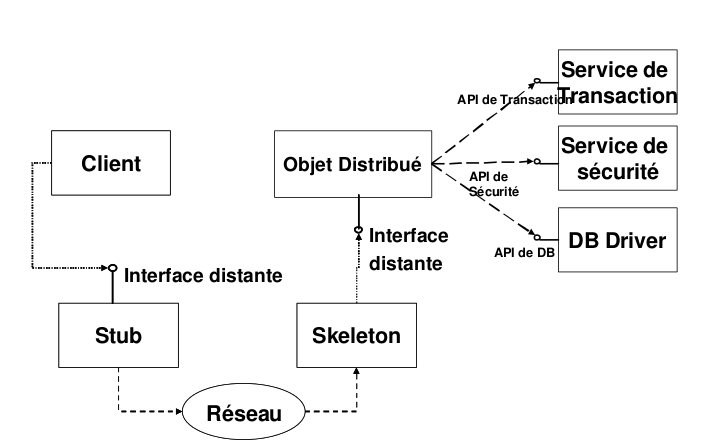
\includegraphics[scale=0.3]{img/ejb-overview.png}
   \end{center}

   \paragraph{} La spécification définit la notion de \textit{bean} - à traduire ici comme
   "conteneur"\footnote{Hé oui, encore un conteneur !}. EJB étant une norme spécifique à Java et à
   la spécification \mylink{TODO}{JEE}, la    notion de \textbf{bean} s'applique en effet à un
   objet\footnote{Pour rappel, un objet est une instanciation en mémoire d'un classe} implémentant une
   fonctionnalité ou un service (technique ou métier) au sein de l'application.

   \paragraph{} En plus de définir un ensemble de caractéristiques spécifiques des \textit{beans},
   la spécification permet de rendre le composant \textbf{local} - c'est à dire s'exécutant au sein
   du même serveur d'application que son client, ou distant de manière complètement transparente.
   Ceci permet donc de séparer, sur des serveurs distincts, des composants ou des traitements
   métiers.

   \paragraph{} En définissant la manière dont ces composants distribués sont utilisées par les
   applications, la spécification permet aussi de décharger ces dernières d'un ensemble de tâches
   techniques (la gestion du cycle de vie du composant ou la sécurisation des échanges par exemple)
   et d'en rendre le serveur d'application responsable. Le respect du standard permettant, en outre,
   de aisément migrer l'application d'un fournisseur de serveur d'application à un autre...\footnote{
   ...Tout du moins en théorie. Il n'est pas si aisé que ça d'effectuer la migration d'une application
   EJB d'un serveur d'application à une autre, mais l'effort nécessaire n'est en rien comparable à ce que
   fût les problèmes de portabilités entre systèmes d'exploitation. À titre d'exemple,
   certaines entreprises ont réussi à migrer d'un serveur JEE à un autre en quelques semaines à peine.}
}

\ifslide{
  \begin{frame}{Exemple de modèle de programmation: EJB}
    \begin{center}
      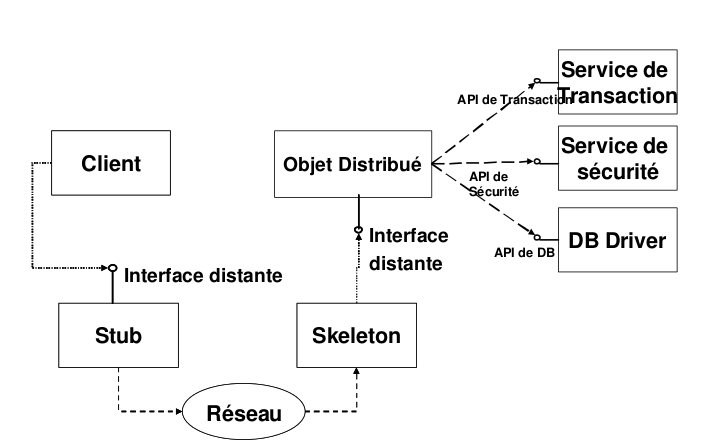
\includegraphics[scale=0.3]{img/ejb-overview.png}
    \end{center}
  \end{frame}

  \begin{frame}
    \begin{block}{Motivations}
      \begin{itemize}
        \item EJB définit des contrats associés à un Bean
        \item Déploiement local ou distant
      \end{itemize}
    \end{block}
  \end{frame}
}

\ifbook{
  \mysubsubsection{Quelques exemples d'EJB}

  \paragraph{} Sans rentrer dans les détails les plus techniques, cette partie va présenter
  quelques caractéristiques que les fameux \textbf{beans} de la spécification EJB peuvent avoir.
  L'analyse de ces quelques caractéristiques devraient en effet éclairer le lecteur sur l'intérêt de
  l'utilisation de cette technologie dans le cadre d'une application, et, par effet de bord,
  l'intérêt de l'utilisation des \textit{frameworks} en général.

  \paragraph{} La norme EJB étant extrêmement vaste et riche, notre présentation se limitera à une
  brève description de certains de ses composants. Nous allons donc étudier les trois types de
  \textbf{beans} suivants:

  \begin{itemize}
    \item \textit{Stateful Bean} et \textit{Stateless Bean}
    \item \textit{Entity Bean}
    \item \textit{Message-Driven Bean}
  \end{itemize}

  \mysubsubsection{Exemple de composant sans ou avec état}

  \paragraph{} Comme décrit plus haut, un composant, au sens EJB, fournit à ses utilisateurs un
  service technique ou métier. Il implémente, pour le compte de l'application, une fonctionnalité
  par exemple. Selon ce traitement, le composant a besoin ou non de conserver un \textbf{état} entre
  chaque requête.

  \paragraph{} Prenons un exemple simple et concret en imaginant un composant dont la charge est de
  vérifier que le mot de passe d'un utilisateur est valide. Selon la manière dont ce mécanisme est
  implémenté, ce composant peut ou non avoir un \textbf{état}.

  \paragraph{} Première implémentation, le composant reçoit une requête avec le nom d'utilisateur et
  le mot de   passe. Il se connecte à un annuaire d'entreprise, probablement par le bais du
  protocole LDAP, vérifie si le mot de passe est correct, ferme la connection et retourne le
  résultat à son composant client.

  \paragraph{} Dans cette première implémentation, le composant est \textbf{sans état} - ou
  \textit{stateless}. En effet, il n'a besoin de ne conserver aucune information entre les requêtes
  qu'il reçoit. Cette même instance peut être utiliser pour une nouvelle requête sans aucun effet de
  bord. En essence, à la fin de la requête, le composant est rigouresement dans le même état
  qu'avant la requête.

  \paragraph{} Modifions maintenant cette implémentation pour lui ajouter un système de cache. En
  effet, comme la communication vers l'annuaire est coûteuse - il s'agit d'un appel réseau après
  tout, il semble pertinent de placer toute information récupérée dans un cache local au composant. À
  chaque requête, le composant vérifiera d'abord si il ne dispose pas de l'information recherchée,
  et sinon, se connectera à l'annuaire. Dans le cas où il disposera déjà de l'information en
  question, le traitement de la requête sera bien évidement beaucoup plus rapide.

  \paragraph{} Cette nouvelle version du composant vient d'introduire un \textbf{état}. Désormais, à
  l'issue d'une requête, il n'est pas garanti que le composant retrouve son état initiale - il peut
  en effet voir son cache augmenté d'une entrée. Le composant est désormais \textit{stateful} et cet
  aspect va grandement modifier la manière dont le serveur applicatif va gérer son cycle de vie.

  \mysubsubsection{Les entités}

  \paragraph{} À la parution de la spécification JEE, ces composants désignés sous le nom de
  \textit{entity beans} ont beaucoup séduit les développeurs et les architectes logicielles. En
  effet, ils portaient avec la eux la promesse de simplifier grandement la gestion d'un aspect
  complexe des applications: la \textbf{persistence}. Si les premières montures de la spécification
  (EJB 1.x et 2.x) sont loin d'avoir tenu ces promesses, la plus récente version (EJB 3.x)
  utilisant le standard JPA facilite réellement la gestion de cette problématique.

  \paragraph{} En effet, un \textbf{entity bean} est un objet conçu pour représenter un ensemble de
  donnée métier. Par exemple, un utilisateur du logiciel (nom, prénom, nom d'utilisateur) ou un
  objet du catalogue, dans le cas d'un site de e-commerce. Cet objet ne contient généralement que
  peu de logique, il se contente de regrouper l'ensemble des attributs de l'entité qu'il représente.

  \paragraph{} Clarifions tout d'abord ce que l'on entend par \textbf{persistance}. Une applications
  Java n'est, au final, qu'un ensemble d'objets instanciés en mémoire. Une partie de ces objets
  représentent souvent des données métiers (les données d'utilisateurs, les produits placés dans le
  panier d'un utilisateur, etc..). Ces informations devant souvent survivre bien au délà de leur
  utilisations par l'application, il est donc nécessaire de le sauvegarder sous une forme durable -
  et non seulement en mémoire.

  \paragraph{} Les bases de données relationnelles, utilisant le langage de requête SQL, sont depuis
  longtemps, à tort ou à raison, devenu l'outil de référence pour confier la persistance des données
  d'une application. Néanmoins, leur modèle de représentation des données - un ensemble de tables
  liées entre elles par des contraintes d'intégrités et des relations, est fondamentalement assez
  différent d'un modèle objets, ou des instances hérites les unes des autres et s'aggrègent.

  \paragraph{} Cette différence profonde est en fait un simple problème \textbf{d'impédance} entre
  la représentation en mémoire des objets et la vision relationnelle des bases de données. Pour
  résoudre ce problème, l'industrie - par le truchement du \textit{framework Open Source}
  \mylink{ToDO}{Hibernate} ou du produit \mylink{}{TopLink}, a souvent eu recours à une approche
  désignée sous le nom de \textit{Object - Relation Mapping (ORM)}.

  \paragraph{} Cette approche est en fait assez simple, elle consiste à fournir à un outil la
  description du travail de transformation à effectuer à partir des objets ou des données issues de
  la base données pour les adapters à la transformation cible. Cet outil allège donc grandement le
  travail des développeurs, pour qui, par exemple, se contente d'invoquer une méthode "sauvegarder"
  pour mettre à jour, en base, un objet qu'ils manipulent.

  \paragraph{} Les outils d'\textit{ORM} prendront en effet à leur charge la gestion de la complexité
  sous jacente du= modèle de données (comme la mise à jour de plusieurs tables si les données de l'objet
  sont sauvegardés sur plusieurs d'entre elles). En outre, effet de bord assez appréciable,
  l'\textit{ORM} fournit une excellente abstraction de la base de données utilisée - abstraction
  standardisée par JPA qui plus est, et permet d'envisager de changer de fournisseur de base de
  données aisément.\footnote{Comme précédemment, on notera que ce genre de migration n'est pas si
  aisée et pose parfois des problèmes, entres autres, de performance. Néanmoins, elles restent tout à
  fait envisageable, dans des délais raisonnables - pour peu que l'application réalisée respecte le
  standard.}

  \paragraph{} Dans le cadre des \textbf{Entity Beans} de EJB 3.x, c'est donc JPA qui est retenu
  pour assurer la persistence des \textbf{Entity Beans}. Comme ces derniers voient leur cycle de vie
  confiés au serveur JEE, le travail des développeurs est encore plus allégé, car ils n'ont même
  plus à déclarer de manière explicite que l'objet doit être mise à jour en base de données - le
  conteneur étant, la plupart du temps, capable de le détecter par lui même !

  \mysubsubsection{Message Driven Bean}

  \paragraph{} Dernier composant issu de la spécification EJB que nous évoquerons dans cette section
  les \textit{Message Driven Bean} (MDB) sont, comme leurs nom anglais l'indique, des composants
  invoqués par le serveur JEE à la réception d'un message transmis par un MOM. L'avantage de ces
  compposants, en plus d'être créer et gérer par le serveur, est qu'ils libèrent le développeur de
  tout la gestion propre à l'utilisation d'un MOM.

}

\ifslide{

  \begin{frame}
    \begin{block}{Standard}
       \begin{itemize}
         \item Portabilité des beans sur différents serveurs EJB
         \item Indépendance du fournisseur
      \end{itemize}
    \end{block}
  \end{frame}

  \begin{frame}
    \begin{block}{Types}
      \begin{itemize}
        \item Session Bean
        \item Entity Bean
        \item Message-Driven Bean
      \end{itemize}
    \end{block}

    \begin{center}
      Si l'on utilise un Session Bean quel impact sur l'architecture de l'application ?
    \end{center}

  \end{frame}
}

\ifbook{
  \mysubsubsection{Synthèse}

  \paragraph{} Sans aller plus loin dans la description des apports de la spécification EJB, dans le
  cadre de développement d'applications JEE, nous pouvons déjà faire une synthèse pédagogique qui
  devrait éclairer le lecteur sur l'intérêt de l'utilisation d'un \textit{framework} et du modèle de
  programmation qu'il promeût.

  \paragraph{} En effet, à la lecture de la description des différents composants évoqués, il
  apparait clairement élégant et avantageux, de les utiliser, si approprié dans le cadre d'un
  développement, pour réduire la quantité de code à produire, et aussi simplifier et standardisé le
  développement. En outre, et c'est là un point crucial, en utilisant un tel \textbf{canevas}, on
  s'assure que les développeurs suivront un modèle de programmation sain et reconnu.

  \paragraph{} Pour illustrer ce point, suppossons qu'une application, réalisée par un développeur
  brillant utilise les éléments suivants:

  \begin{itemize}
    \item un ensemble de service, avec ou sans état, mais ne suivant pas le standard EJB
    \item certains traitements sont déclenché lors de la réception de message provenant d'un MOM, mais
    l'implémentation ne suit pas la norme des MDB.
    \item la persistance est réalisée de manière spécifique, utilisant simplement des requêtes SQL,
    directement executées sur la base de données.
  \end{itemize}

  \paragraph{} Une telle application, en plus de problème de poser potentiellement des problèmes de
  configuration et d'adhérence à la base de données utilisée, posent aussi un problème encore plus
  pragmatique : le recrutement de développeurs pour travailler dessus. Seul un développeur brillant et
  maitrisant les différentes techniques utilisées par le concepteur original sera en mesure
  d'assurer la maintenance du code et l'ajout de nouvelles fonctionnalités.

  \paragraph{} À l'inverse une application JEE standard pourra non seulement être maintenue par la
  plupart des développeurs de l'industrie, pour peu qu'il soit famillié avec le standard, et pourra
  être optimisée lors de son déploiement, à l'aide des nombres aspects de son fonctionnement qui ont
  été déportés vers le serveur JEE.

  \paragraph{} Cette conclusion n'est évidement par propre au standard EJB. Elle s'applique à
  l'utilisation du célèbre \textit{framework} \mylink{TODO}{Spring} ou encore dans le monde Ruby, de
  \mylink{TODO}{Ruby On Rails}. Ce qui est essentiel de retenir c'est qu'un modèle de programmation
  - apporté par un \textit{framework}, permet d'accéler et de faciliter grandement le développement
  d'application.

  \paragraph{} Néanmoins, il faut aussi retenir que leur utilisation est très \textbf{structurante}
  et que si ils ne sont pas donc pas adaptés au besoin de l'application, ils peuvent devenir une
  entrâve, en empêchant littéralement le développeur de réaliser les fonctionnalités demandées.
}
